\documentclass[11pt]{article}
\usepackage[a4paper,margin=24mm]{geometry}
\usepackage{amsmath,amssymb}
\usepackage{booktabs}
\usepackage{makecell}
\renewcommand\theadfont{\normalfont}\renewcommand\theadalign{rb}
\usepackage{graphicx}
\usepackage{microtype}
\usepackage[hidelinks]{hyperref}
\usepackage{xcolor}
\usepackage{caption}
\captionsetup{font=small,labelfont=bf}
\setlength{\parskip}{3pt}
\newcommand{\hm}{h-means}
\newcommand{\emeans}{e-means}
\newcommand{\nk}{n/k}
\newcommand{\norm}[1]{\lVert #1 \rVert}

\title{\hm: mini-batch $k$-means with a hierarchical warm start\\and Hartigan assignment}
\author{Hélder Monteiro}
\date{November 2026\thanks{Technical note accompanying the \texttt{hmeans} repository: \url{https://github.com/heldernoid/hmeans}. Code, logged runs, the scripts that regenerate every table, and a browser playground.}}

\begin{document}
\maketitle

\begin{abstract}
\emeans{} (Bessa et al., 2026) trains $k$-means on mini-batches with an exponential moving average of cluster statistics and reaches a lower loss than Lloyd's algorithm in a tenth of the passes over the data. We keep its update, batch and step-size laws, schedule and dead-cluster revival, and change two things: the initialisation, which becomes a hierarchical warm start whose allocation of centroids follows the loss, and the assignment rule, which becomes Hartigan's exact move criterion in place of nearest-centroid assignment, written as one matrix product so that it costs the same. On SIFT, GloVe, NYTimes, Fashion-MNIST and two synthetic mixtures, at equal distance computations, the resulting method (\hm) reaches 2 to 7\% lower $k$-means loss than the better of \emeans's two batch laws whenever clusters hold 20 points or fewer, on every configuration and every seed, with 3 to 10 times smaller seed variance; it matches \emeans{} within $\pm0.03\%$ at hundreds of points per cluster and is 0.2\% better on a 10M-row run. Held-out gains are about a fifth of the training gains. An ablation attributes the gain to Hartigan's $N/(N\pm1)$ factors, not to exact bookkeeping, and to the loss-proportional allocation of the warm start on imbalanced data. We also report the approximate-assignment ideas that did not work and state the limitations, including that the one tunable of the method, the fraction of passes run in mini-batch mode, was set on the reported grid. Code, logs and an interactive playground are at \url{https://github.com/heldernoid/hmeans}.
\end{abstract}

\section{Introduction}

$k$-means with large $k$ is the workhorse of vector quantisation and of inverted-file indexes for nearest-neighbour search. Lloyd's algorithm costs one full pass of $n k$ distance computations per iteration and is typically run for 20 to 50 iterations. \emeans{} \cite{emeans} showed that a mini-batch method with an exponential moving average (EMA) of per-cluster statistics, batch sizes and step sizes set by fitted laws, a cosine schedule and periodic revival of dead clusters, reaches a lower loss than Lloyd at 25 iterations after 3 to 5 passes. Its authors ship the recipe in faiss and fit its laws for $\nk \ge 8$.

Reproducing \emeans{} (Section~\ref{sec:repro}) we found that it is not converged at 5 passes, that its smaller-batch ``quality'' law is better than the default on our hardware, and that its margin over Lloyd shrinks and reverses as clusters get small: at seven points per cluster Lloyd at 25 iterations beats it. Small clusters are where the mini-batch estimate of a cluster's size and position is noisiest, and where nearest-centroid assignment makes moves that increase the objective.

\hm{} addresses that regime with two changes (Section~\ref{sec:method}). Everything else is \emeans. With the changes switched off, our implementation reproduces the official code within seed noise.

\paragraph{In one paragraph.} \emeans{} starts from $k$ random rows; \hm{} first runs half a pass of \emeans{} with $k/16$ coarse centroids, splits each coarse cluster into children in proportion to its share of the loss, and places the children with two local Lloyd iterations, for about a tenth of a pass. \emeans{} assigns each point to its nearest centroid; \hm{} moves a point from cluster $a$ to $b$ only if $\frac{N_a}{N_a-1}\,d^2(x,a) > \frac{N_b}{N_b+1}\,d^2(x,b)$, the exact change of the objective for one move, using the EMA mass as the size estimate during the mini-batch passes and exact counts in optional exact passes at the end. The share of the budget given to the exact passes decreases with points per cluster, because exact passes only make local moves.

\section{Background: \emeans{}}
\label{sec:emeans}

All methods here keep a sum $S_j$ and a count $N_j$ per cluster and take $c_j = S_j/N_j$. Lloyd recomputes both from the whole data at every iteration. \emeans{} processes mini-batches of $B$ points; with $n_j$ the number of batch points assigned to cluster $j$ and $m_j$ their mean, the update is
\begin{equation}
N_j \leftarrow (1-\alpha)\,N_j + \alpha\, n_j, \qquad c_j \leftarrow c_j + \frac{\alpha\, n_j}{N_j}\,(m_j - c_j),
\end{equation}
with $\alpha$ following a cosine schedule from a peak $\alpha_0$ to a tenth of it. $B$ and $\alpha_0$ are set by laws of $k$, $n$ and the number of passes $T$ (constants as shipped in faiss):
\begin{equation}
B = C_B\, k^{0.135}\, n^{0.876}\, T^{0.813}, \qquad \alpha_0 = 0.824\, k^{-0.462}\, B^{0.900}\, n^{-0.450}\, T^{-0.106},
\end{equation}
with $C_B = 0.0351$ (throughput law) or eight times smaller (quality law). Every five updates, clusters whose mass is below a tenth of the mean are revived by splitting a donor sampled in proportion to mass. After the last pass the centroids are replaced by the exact means of the points seen during that pass.

\section{Reproduction of \emeans{}}
\label{sec:repro}

We reimplemented \emeans{} in PyTorch on a shared exact-assignment backend (chunked matrix product and argmin) so that all methods share the same assignment code, initial rows, evaluation and operation counting. The reimplementation matches the official faiss \texttt{NumpyEmeans} within seed noise on SIFT and GloVe (CPU cross-check in Section~\ref{sec:cpu}). Four observations shaped the work. (i) \emeans{} at three passes beats Lloyd at 25 iterations on every dataset we tried. (ii) It is not converged at five passes: the loss keeps decreasing to 25. (iii) The quality law (eight times smaller batches) is 0.2 to 1.5\% better than the default throughput law at equal passes on our hardware; we report both and compare against the better one. (iv) At small $\nk$ the margin disappears: on NYTimes with $k=32{,}768$ (seven points per cluster) Lloyd at 25 iterations is 1.4\% better than \emeans{} at five passes. Finishing \emeans{} with exact Lloyd passes recovers only about 0.1\%.

\section{Method}
\label{sec:method}

\subsection{Hierarchical warm start with loss-proportional allocation}

Run \emeans{} for half a pass with $k_c = k/16$ coarse centroids from random rows. Assign every point to its coarse centroid (cost $n k_c$, a sixteenth of a pass) and accumulate each coarse cluster's count $|C_j|$ and sum of squared errors $\mathrm{SSE}_j$. Apportion the $k$ fine centroids to the coarse clusters by largest remainder,
\begin{equation}
k_j = \operatorname{apportion}\Big(k\cdot \frac{\mathrm{SSE}_j}{\sum_i \mathrm{SSE}_i}\Big), \qquad 1 \le k_j \le |C_j|,
\end{equation}
start the children at random members of their coarse cluster, and run two Lloyd iterations in which a point only sees the $k_j$ children of its own coarse cluster (cost $2 n k / k_c$, an eighth of a pass). Each child's EMA mass is initialised to its count scaled to one batch, $N_j = |C_j^{\mathrm{child}}|\,B/n$, so the first mini-batch updates neither ignore nor over-trust the warm start. A uniform allocation instead of the loss-proportional one is 9.5\% worse on an imbalanced mixture (Section~\ref{sec:ablation}).

\subsection{Hartigan's move rule as a matrix product}

Moving one point $x$ from cluster $a$ (size $N_a$) to cluster $b$ (size $N_b$) changes the $k$-means objective by exactly \cite{hartigan}
\begin{equation}
\Delta_{a\to b}(x) = \frac{N_b}{N_b+1}\,\norm{x - c_b}^2 - \frac{N_a}{N_a-1}\,\norm{x - c_a}^2 .
\end{equation}
The point moves to the $b$ that minimises its join cost if that is below its stay cost. Lloyd's rule is the limit of both factors going to one; at ten points per cluster they are $0.91$ and $1.11$. With $g_j = N_j/(N_j+1)$ the join costs of all centroids are a product of augmented vectors,
\begin{equation}
g_j\,\norm{x - c_j}^2 = \big[\,\norm{x}^2,\; x,\; 1\,\big]\cdot\big[\,g_j,\; -2 g_j c_j,\; g_j \norm{c_j}^2\,\big],
\end{equation}
so a batch against all $k$ centroids is one matrix product in $d+2$ dimensions instead of $d$, followed by writing each point's stay cost into its current column and an argmin. Empty clusters cannot be joined through the rule (their join cost is infinite; a first version without this guard collapsed) and are re-seeded at the farthest point of a mass-sampled donor every five updates.

\subsection{Where the rule runs}

Inside the EMA passes the rule uses the size estimate $\hat N_j = N_j\, n/B$, the EMA mass being a per-batch quantity. After the EMA passes, optional exact passes maintain the exact sums and counts of all points (available for free from the last EMA pass) incrementally as points move, re-assigning each batch with the same rule; every update is then an exact partial Lloyd step and the objective is monotone. With $T$ total passes the first $\max(1,\operatorname{round}(f T))$ are EMA passes. The fraction $f$ depends on points per cluster: $0.4$ below 24, $0.8$ below 64, $1.0$ (no exact passes) above. Exact passes only make local moves; with few points per cluster that is what is needed, with many the warm start carries the gain and further EMA passes keep it better than exact passes do (Section~\ref{sec:sweep}). The dead-cluster donor may also be sampled in proportion to a cluster's running SSE instead of its mass; this has no measurable effect and is not part of the claim.

\section{Experiments}

\subsection{Protocol}

One machine (Apple M3 Ultra; PyTorch on the GPU through MPS, and on 32 CPU cores for the timing cross-check). Datasets: SIFT-128 (980k rows), GloVe-100 (1.16M, $L_2$-normalised), NYTimes-256 (229k, normalised), Fashion-MNIST-784 (40k), two 96-dimensional Gaussian mixtures of 500k rows (balanced with 4,096 components; Zipf-imbalanced with 2,048), and Deep-96 (9.97M). 20,000 rows are held out per dataset. $k$ ranges from $\nk \approx 120$ down to $\nk \approx 7$. Baselines: Lloyd at 25 iterations from random rows (3 seeds); greedy $k$-means++ seeding (50k sample, 3 trials; once on the full data) followed by Lloyd at 25; Sculley's mini-batch $k$-means \cite{sculley} ($B=4096$, 5 passes); \emeans{} at 3 and 5 passes with its default law and at 5 passes with its quality law (5 seeds). \hm{} at 3 and 5 passes in total, the warm start's $\approx 0.1$ pass counted. Metrics: exact training MSE on all rows, exact held-out MSE, wall-clock of \texttt{fit}, and distance computations in units of $nk$ (``passes''). ``Best \emeans'' means the better of its two laws per configuration.

\paragraph{Recipe selection.} Three fixed recipes were run on the full grid in this order: v1 (no Hartigan correction inside the EMA passes), v2 (Hartigan-EMA, $f=0.8$), v3 (Hartigan-EMA, $f=0.4$). v3 won below 20 points per cluster, v2 between 30 and 60, and both lost a quarter percent above 120; a synthetic check at 234 points per cluster then showed the exact tail itself losing the warm start's gain. The final rule for $f$ was set from these results, and ``\hm'' below is that rule applied to the logged runs plus 58 later runs with $f=1.0$ on the large-$\nk$ configurations. The thresholds were chosen on the grid we report; there is no held-out set of configurations.

\subsection{Main comparison}

\begin{table}[t]
\centering\small
\caption{Training MSE of \hm{} at 5 passes relative to the best \emeans{} at 5 passes (mean of 5 seeds; $\pm$ is the seed std of \hm{} as a percentage of the \emeans{} mean), relative to \emeans's default law, \hm{} at 3 passes relative to the best \emeans{} at 5, and the number of seeds on which \hm{} is below the \emeans{} mean. Negative is \hm{} better.}
\label{tab:main}
\small
\begin{tabular*}{\textwidth}{@{\extracolsep{\fill}}lrrrrrr@{}}
\toprule
\thead[lb]{dataset} & $k$ & $\nk$ & \thead{\hm{} T5 vs\\best \emeans{} T5} & \thead{\hm{} T5 vs\\default law} & \thead{\hm{} T3 vs\\best \emeans{} T5} & \thead{seeds\\won} \\
\midrule
Fashion-MNIST-784 & 512 & 78 & $-0.35\%$ ($\pm0.04$) & $-0.52\%$ & $+0.01\%$ & 5/5 \\
Fashion-MNIST-784 & 2,048 & 20 & $-2.19\%$ ($\pm0.04$) & $-2.53\%$ & $-1.49\%$ & 5/5 \\
GloVe-100 & 16,384 & 71 & $-0.03\%$ ($\pm0.01$) & $-0.22\%$ & $+0.37\%$ & 5/5 \\
GloVe-100 & 65,536 & 18 & $-2.02\%$ ($\pm0.01$) & $-2.57\%$ & $-1.21\%$ & 5/5 \\
GloVe-100 & 131,072 & 9 & $-4.44\%$ ($\pm0.02$) & $-5.74\%$ & $-3.65\%$ & 5/5 \\
NYTimes-256 & 4,096 & 56 & $-0.46\%$ ($\pm0.02$) & $-0.59\%$ & $+0.04\%$ & 5/5 \\
NYTimes-256 & 16,384 & 14 & $-3.15\%$ ($\pm0.08$) & $-4.96\%$ & $-2.43\%$ & 5/5 \\
NYTimes-256 & 32,768 & 7 & $-6.70\%$ ($\pm0.34$) & $-9.66\%$ & $-5.94\%$ & 5/5 \\
SIFT-128 & 16,384 & 60 & $-0.24\%$ ($\pm0.00$) & $-0.43\%$ & $+0.46\%$ & 5/5 \\
SIFT-128 & 65,536 & 15 & $-2.26\%$ ($\pm0.01$) & $-3.07\%$ & $-0.97\%$ & 5/5 \\
SIFT-128 & 131,072 & 7 & $-5.97\%$ ($\pm0.01$) & $-7.26\%$ & $-4.27\%$ & 5/5 \\
GMM-Zipf ($d=96$) & 4,096 & 122 & $-2.16\%$ ($\pm0.17$) & $-2.16\%$ & $-1.92\%$ & 5/5 \\
GMM-Zipf ($d=96$) & 16,384 & 31 & $-0.89\%$ ($\pm0.00$) & $-1.02\%$ & $-0.57\%$ & 5/5 \\
GMM ($d=96$) & 8,192 & 61 & $-0.18\%$ ($\pm0.02$) & $-0.18\%$ & $-0.08\%$ & 5/5 \\
GMM ($d=96$) & 32,768 & 15 & $-1.62\%$ ($\pm0.00$) & $-1.62\%$ & $-1.29\%$ & 5/5 \\
\bottomrule
\end{tabular*}
\end{table}

\begin{figure}[t]
\centering
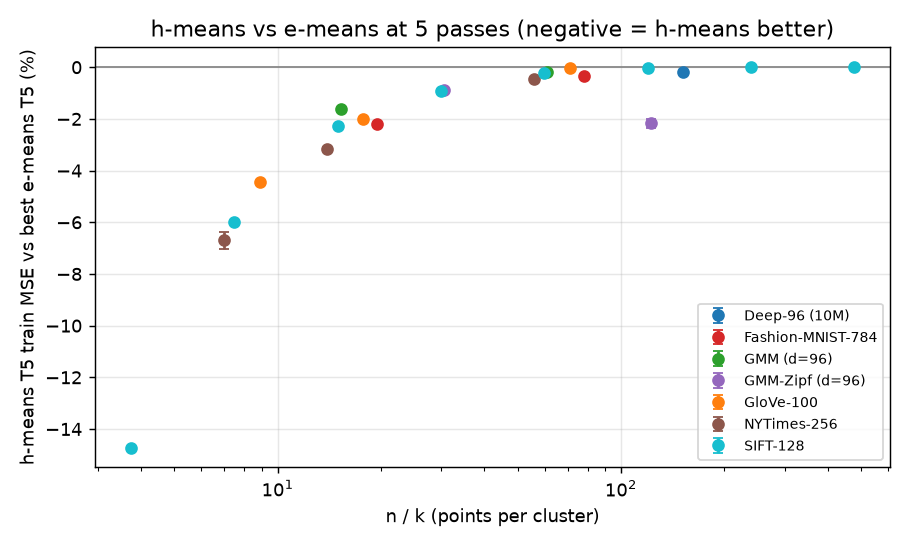
\includegraphics[width=0.78\linewidth]{figures/wins_vs_nk.png}
\caption{Training MSE of \hm{} at 5 passes relative to the best \emeans{} at 5 passes, against points per cluster, all configurations of Table~\ref{tab:main}. Error bars: one seed standard deviation.}
\label{fig:wins}
\end{figure}

Table~\ref{tab:main} and Figure~\ref{fig:wins} give the main result. The gain is a function of points per cluster: 0.03 to 0.5\% at $\nk \approx 60$ to 80, 1 to 2.5\% at 15 to 20, 4.5 to 7\% at 7 to 9. \hm{} is below the best \emeans{} on all 15 configurations and all 75 seed runs; the smallest margin, GloVe at $k=16{,}384$, is within one seed standard deviation of a tie. At $\nk \le 20$, \hm{} after three passes is already below \emeans{} after five (1.0 to 5.9\%). The seed standard deviation of \hm{} is typically 3 to 10 times smaller than that of \emeans{} with its default law. The baselines behave as published: \emeans{} at five passes beats Lloyd at 25 by 0.7 to 3\% except at NYTimes $k=32{,}768$, where Lloyd is 1.4\% better than \emeans{} and \hm{} is 8.4\% better than Lloyd; Sculley is 1.4 to 19\% worse than \emeans; $k$-means++ seeding plus Lloyd at 25 is 0.5 to 1.3\% worse than \emeans{} at five passes and 50 to 100 times slower, and seeding on the full SIFT data (419\,s of seeding alone) is still 0.7\% above \emeans{} at five passes.

\subsection{Held-out loss}

\hm{} optimises the training objective and the held-out picture is weaker. Held-out MSE of \hm{} at 5 passes against the best \emeans{} is lower on 11 of 15 configurations (from $-0.03\%$ to $-2.15\%$), within $\pm0.05\%$ on two, and higher on GloVe $k=16{,}384$ ($+0.12\%$) and on the balanced synthetic mixture at 15 points per cluster ($+0.70\%$), where the exact passes fit the training rows of a perfectly separable problem. On the real datasets the held-out gain tracks the training gain at about a fifth of its size.

\subsection{Dependence on $k$, and large data}
\label{sec:sweep}

\begin{table}[t]
\centering\small
\caption{SIFT-128, $n=980{,}000$, five passes, three seeds. Training MSE (mean $\pm$ std) and the time of \texttt{fit} on the GPU.}
\label{tab:sweep}
\small
\begin{tabular*}{\textwidth}{@{\extracolsep{\fill}}rrrrrrr@{}}
\toprule
$k$ & $\nk$ & \thead{\emeans{} T5\\(default law)} & \thead{\emeans{} T5\\(quality law)} & \thead{\hm{} T5} & \thead{\hm{}\\vs best} & \thead{time (s)\\\emeans{} / \hm{}} \\
\midrule
2,048 & 479 & 47239 $\pm$ 4 & 47200 $\pm$ 5 & 47213 $\pm$ 2 & $+0.03\%$ & 0.7 / 2.6 \\
4,096 & 239 & 44192 $\pm$ 5 & 44148 $\pm$ 3 & 44157 $\pm$ 2 & $+0.02\%$ & 1.0 / 2.9 \\
8,192 & 120 & 41113 $\pm$ 8 & 41051 $\pm$ 2 & 41040 $\pm$ 2 & $-0.03\%$ & 1.5 / 3.4 \\
16,384 & 60 & 37831 $\pm$ 2 & 37757 $\pm$ 1 & 37668 $\pm$ 1 & $-0.24\%$ & 2.6 / 3.6 \\
32,768 & 30 & 34185 $\pm$ 9 & 34024 $\pm$ 1 & 33705 $\pm$ 4 & $-0.94\%$ & 4.5 / 6.1 \\
65,536 & 15 & 29718 $\pm$ 16 & 29480 $\pm$ 2 & 28809 $\pm$ 4 & $-2.28\%$ & 15.1 / 15.5 \\
131,072 & 7 & 23996 $\pm$ 49 & 23681 $\pm$ 5 & 22264 $\pm$ 1 & $-5.98\%$ & 30.4 / 29.1 \\
262,144 & 4 & 16714 $\pm$ 68 & 16448 $\pm$ 10 & 14026 $\pm$ 0 & $-14.73\%$ & 60.0 / 67.1 \\
\bottomrule
\end{tabular*}
\end{table}

Table~\ref{tab:sweep} sweeps $k$ at fixed $n$. Above two hundred points per cluster \hm{} ($f=1.0$ there) ties \emeans's quality law within $\pm0.03\%$ and is 0.05 to 0.2\% below its default law; from sixty points per cluster down the gap widens to 15\% at four points per cluster, where Lloyd's algorithm is itself competitive with \emeans. With a fixed $f=0.4$ the large-$k$ end was $+0.25\%$ and the small end $-14.7\%$; with a fixed $f=0.8$, $+0.07\%$ and $-7.4\%$. On Deep-96 with 9.97M rows and $k=65{,}536$ (152 points per cluster, the inverted-file regime, two seeds) \hm{} is 0.20\% below \emeans{} at five passes in 135\,s against 151\,s, with held-out MSE 0.15\% lower; Lloyd at 25 iterations is 0.5\% above \emeans{} in 733\,s.

\subsection{Wall-clock}
\label{sec:cpu}

Distance computations are the hardware-independent comparison; wall-clock depends on the implementation. On the GPU, at equal passes, \hm{} is 10 to 15\% faster than \emeans{} on the problems that take more than 15\,s (the exact passes use fewer, larger kernels) and two to five times slower on sub-5-second problems, where the warm start and the per-batch bookkeeping are fixed costs (Table~\ref{tab:sweep}, last column). On 32 CPU cores with the same torch backend (three seeds; timings carry about $\pm10\%$ noise from concurrent jobs), at $k=65{,}536$ \hm{} after three passes reaches a lower loss than \emeans{} after five in about half the time: SIFT 29191 in 40.6\,s against 29718 in 78.7\,s; GloVe 0.4720 in 59\,s against 0.4805 in 99\,s. The official faiss implementation reaches the same loss as our \emeans{} (29719 against 29718) in 304\,s, its assignment going through \texttt{faiss.knn} rather than a BLAS product.

\subsection{Ablation}
\label{sec:ablation}

\begin{table}[t]
\centering\small
\caption{Each component switched off in turn, five passes, five seeds. Training MSE relative to the recipe with the fixed $f=0.4$ (the rule's choice at 15 and 18 points per cluster); negative is better than it.}
\label{tab:ablation}
\small
\begin{tabular*}{\textwidth}{@{\extracolsep{\fill}}lrrrr@{}}
\toprule
\thead[lb]{variant} & \thead{GloVe 65k\\($\nk = 18$)} & \thead{SIFT 65k\\($\nk = 15$)} & \thead{SIFT 16k\\($\nk = 60$)} & \thead{GMM-Zipf 4k\\($\nk = 122$)} \\
\midrule
full ($f=0.4$) & 0 & 0 & 0 & 0 \\
$-$ SSE donors (mass donors) & $-0.00\%$ & $+0.00\%$ & $+0.00\%$ & $-0.01\%$ \\
$-$ SSE allocation (uniform children) & $+0.08\%$ & $+0.11\%$ & $+0.01\%$ & $\mathbf{+9.46\%}$ \\
$-$ Hartigan in EMA passes & $+0.16\%$ & $+0.37\%$ & $+0.07\%$ & $-0.01\%$ \\
$-$ warm start & $+0.56\%$ & $+0.61\%$ & $+0.20\%$ & $+2.78\%$ \\
$-$ exact tail (EMA only, same passes) & $+1.61\%$ & $+1.50\%$ & $-0.24\%$ & $-0.24\%$ \\
$-$ Hartigan rule in tail (Lloyd-rule tail) & $+2.31\%$ & $+2.64\%$ & $+0.55\%$ & $+0.22\%$ \\
$f = 0.8$ & $+0.64\%$ & $-0.08\%$ & $-0.25\%$ & $-0.28\%$ \\
$f = 1.0$ & $+1.61\%$ & $+1.50\%$ & $-0.24\%$ & $-0.31\%$ \\
\emeans{} + Hartigan-EMA only & $+1.91\%$ & $+2.17\%$ & $-0.14\%$ & $+1.89\%$ \\
\emeans{} (all off) & $+2.64\%$ & $+3.19\%$ & $+0.18\%$ & $+2.08\%$ \\
\bottomrule
\end{tabular*}
\end{table}

Table~\ref{tab:ablation}: the exact Hartigan tail is the largest single lever at small $\nk$ (1.5 to 1.6\%), and it is the $N/(N\pm1)$ rule rather than the exact bookkeeping that matters, since a Lloyd-rule tail with identical bookkeeping is 2.3 to 2.6\% worse than the Hartigan tail and worse than no tail. The warm start is worth 0.2 to 2.8\%, most on the imbalanced mixture, and its loss-proportional allocation is what survives imbalance. Hartigan-corrected assignment inside the EMA passes adds 0.1 to 0.4\% at small $\nk$ and nothing at 60. The split is regime-dependent, which is what the rule for $f$ encodes: at 15 to 18 points per cluster $f=0.4$ is best or within 0.1\% of best; at 60 and 122 the larger fractions are 0.25 to 0.3\% better and indistinguishable from each other.

\section{What did not work}

Several ideas to make assignment cheaper than one dense product were tried first and are recorded because they are the natural things to try. A cached candidate list per point (re-score only the few nearest centroids of the previous visit) and a centroid $k$-NN graph with local search both miss near-ties on real embeddings and stall above exact assignment. Triangle-inequality bounds certify only 0.1\% of the distance computations in 128 dimensions. PCA filter-and-refine costs at least twice the multiply-adds of one product and is slower on an accelerator. An inverted-file first pass, growing batch sizes and a Lloyd-rule incremental tail did not move the loss at equal passes.

\section{Limitations}

\begin{itemize}\setlength{\itemsep}{1pt}
\item \textbf{Regime.} The clear wins are a small-cluster effect. In the inverted-file regime of hundreds of points per cluster \hm{} is a tie to a small win. Where it wins by 5 to 7\%, Lloyd at 25 iterations is also competitive with \emeans.
\item \textbf{Held-out.} Training gains carry to held-out loss at about a fifth of their size and can reverse on separable synthetic data at 15 points per cluster.
\item \textbf{Selection.} The rule for $f$ and the recipe were chosen after seeing the grid. Table~\ref{tab:main} is ``best of three measured splits'' per configuration rather than one pre-registered recipe; all fixed-recipe rows are in the repository, and the ablation shows the 0.4 and 0.8 splits within 0.1\% at 15 points per cluster and 0.6\% apart at 18, so the lower threshold is soft. A held-out set of datasets would settle it and was not run. For the user, \hm{} takes the same two inputs as \emeans, $k$ and the pass budget: batch and step sizes follow the \emeans{} laws and the coarse level ($k/16$), the two local Lloyd iterations and the EMA constants are fixed. The one method constant \emeans{} does not have, the rule for $f$, was however set on the grid we evaluate, whereas the \emeans{} laws were fitted on a dedicated sweep and evaluated elsewhere; Deep-10M and the ends of the SIFT sweep, run after the rule was fixed, are its only out-of-sample checks.
\item \textbf{Wall-clock at small scale} and \textbf{one machine}: see Section~\ref{sec:cpu}. A CUDA comparison against the official implementation was not possible here.
\item \textbf{Memory.} The exact passes keep one label per point and the exact per-cluster sums; \emeans{} keeps only the centroids.
\end{itemize}

\section{Conclusion}

\emeans{} plus a loss-proportional hierarchical warm start and Hartigan's $N/(N\pm1)$ correction is a strictly better optimiser of the $k$-means objective when clusters are small, and the same algorithm when they are not. The correction costs nothing extra, the warm start costs a tenth of a pass, and the implementation is a drop-in with a scikit-learn interface on NumPy or PyTorch. The repository contains the logged runs behind every number here, the scripts that regenerate the tables, and a browser playground in which the three methods run on the same points at the same number of distance computations.

\section*{Acknowledgements}
Claude Fable 5.1 (Anthropic) assisted with the experiment design, the automation of the runs and the drafting of this note. The method, the choices made on the way and the responsibility for the results are the author's.

\begin{thebibliography}{9}
\bibitem{emeans} L. Bessa et al. e-means: outperforming $k$-means in one-tenth the epochs. arXiv:2611.09501, 2026. Code in faiss, \texttt{contrib/e\_means}; site \url{https://e-means.github.io}.
\bibitem{hartigan} J. A. Hartigan and M. A. Wong. Algorithm AS 136: A $k$-means clustering algorithm. \emph{Applied Statistics} 28(1):100--108, 1979.
\bibitem{lloyd} S. P. Lloyd. Least squares quantization in PCM. \emph{IEEE Transactions on Information Theory} 28(2):129--137, 1982.
\bibitem{sculley} D. Sculley. Web-scale $k$-means clustering. \emph{WWW}, 2010.
\bibitem{kmpp} D. Arthur and S. Vassilvitskii. $k$-means++: the advantages of careful seeding. \emph{SODA}, 2007.
\end{thebibliography}

\end{document}
